\documentclass[12pt]{article}
\usepackage[margin=1in]{geometry}
\usepackage{amsmath}
\usepackage{graphicx}
\usepackage{setspace}
\usepackage{subcaption}
\usepackage{listings}
\usepackage[italicdiff]{physics}
%\usepackage{natbib}
\usepackage{epstopdf}
\lstset{breaklines=true, tabsize = 3}
\usepackage[american]{babel}
\usepackage[babel]{csquotes}
\usepackage[notes,backend=biber]{biblatex-chicago}
\addbibresource{nbody.bib}
\author{Jonathan Bunton}
\title{Modeling Atomic Interactions in Xenon \\ Using the Morse and Lennard-Jones Potentials with \\
Fourth-Order Runge-Kutta Integration}
\date{\today}

\begin{document}
\maketitle
\onehalfspacing
\begin{abstract}
Inter-atomic forces are often modeled using potential well models, characterized by an attractive long range force and a stronger repulsive short range force.   Two such models are the Lennard-Jones and Morse potentials, each of which exhibit this behavior with differing mathematical premises.  The Lennard-Jones potential accomplishes this with two terms:
\begin{equation*}
U(r) = \varepsilon\left[ \left( \frac{r_m}{r} \right)^{12}-2\left(\frac{r_m}{r}\right)^6\right]
\end{equation*}
Here $r$ is the distance between particles, and the parameters $\varepsilon$ and $r_m$ determine the depth of the potential curve and its lowest point respectively. \autocite{ljpotential} The parameters for these values are characteristic to a material, in this paper's case, Xenon.  The Morse potential achieves a similar shape using exponentials:
\begin{equation*}
U(r) = D_e \left(1-e^{-a(r-r_e)}\right)^2
\end{equation*}
In the Morse potential, the parameters $D_e$ and $a$ control the depth and width of the potential well respectively, while $r_e$ is the lowest point. \autocite{mpotential}  Again these coefficients are characteristic of the material, Xenon for this paper.   Despite very different mathematical formulation, these potentials have very similar shapes.

This paper analyzes the behavior of a lattice of Xenon atoms in both the Lennard-Jones and the Morse potentials by using fourth-order Runge-Kutta (RK4) integration methods to numerically calculate the equations of motion for the system. \autocite{rk4} The coefficients for these potentials are experimentally determined from the second virial coefficient. \autocite{mconstants, ljconstants}  Fourth-order Runge-Kutta shows high precision, at the cost of computation time.  Compared to a simpler method, such as Verlet integration, our data shows an average of a 300\% increase in calculation time from Verlet integration to RK4. 
As expected, the simulation data also exhibits the spring-esque behavior suggested by the potential wells, as well as increased evaporation and decreased order with a higher temperature.
\end{abstract}
\section*{Results}
Both the Lennard-Jones and Morse potentials were simulated using code developed in previous assignments, tailored to the RK4 algorithm.  This code initializes the velocities in each direction using the Maxwell-Boltzmann distribution in each dimension.  

As was shown in the case of Verlet integration, the system proved semi-stable for both potentials, with a slight oscillatory behavior as expected from the potential shapes.  Ultimately, the steady-state solution appeared to be a sphere, where each particle is spaced at an adequate distance to be "trapped" in the curve of the potential well.  In addition, at lower temperatures clusters appear where groups of particles sit in the minimum potential position ($r_m$ or $r_e$) in smaller groups after leaving the larger initial lattice.

Computationally, the data shows a more precise conservation of energy and momentum, both of which ought to remain constant throughout calculations.  Variation in energy through 10000 timesteps of $10^{-14}$ is on the order of 0.001\% and $< 10^{-10}$\% in momentum.  The error of the RK4 algorithm appears to lose total energy slightly through iterations, which is likely caused by low roundoff errors over the averaging period and numerical issues involving time step size selection.  Because momentum and energy are conserved so incredibly precisely, we can consider RK4 a valid numerical approximation method for this system.

\subsection*{Lennard-Jones Potential}
The Lennard-Jones (6-12) potential creates a semi-stable system.  Our simulation results conserve energy and momentum while settling into a steady state orientation, provided a small enough time-step (in this case $10^{-14}$ seconds).  This is shown most clearly by the stability of the graphs in figs. \ref{LJEconservation} and \ref{LJPconservation}, which  exhibit a deviation on the order of 0.001\% in total energy and $< 10^{-10}$\% in total momentum.  These percentages hold for timesteps of $10^{-14}$, but smaller timesteps of course provide higher precision.  Conversely, larger timesteps result in too drastic of changes in the system between timestep iterations for momentum and energy to be effectively conserved.

%L-J CONSERVATION PICS
\begin{figure}[!h]
\begin{subfigure}{0.5\textwidth}
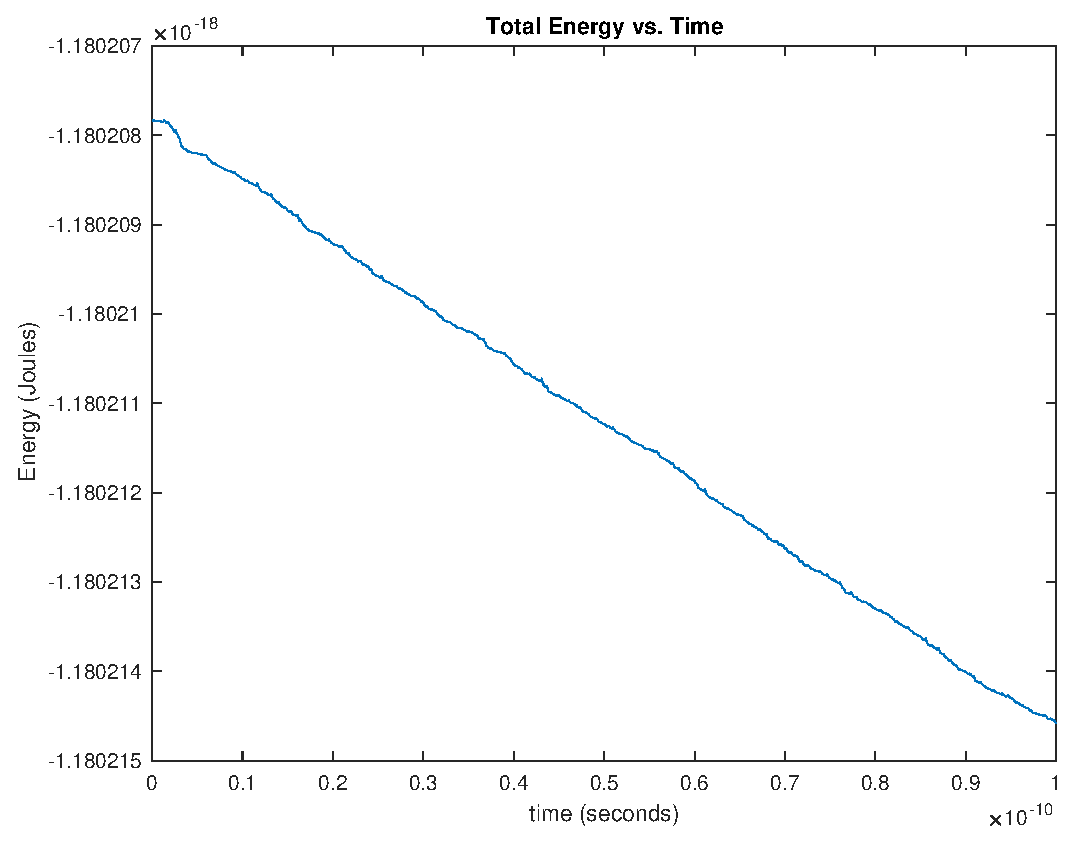
\includegraphics[width=0.9\linewidth]{./finalpics/LJEvsT.eps}
\caption{\label{LJEconservation}}
\end{subfigure}
\begin{subfigure}{0.5\textwidth}
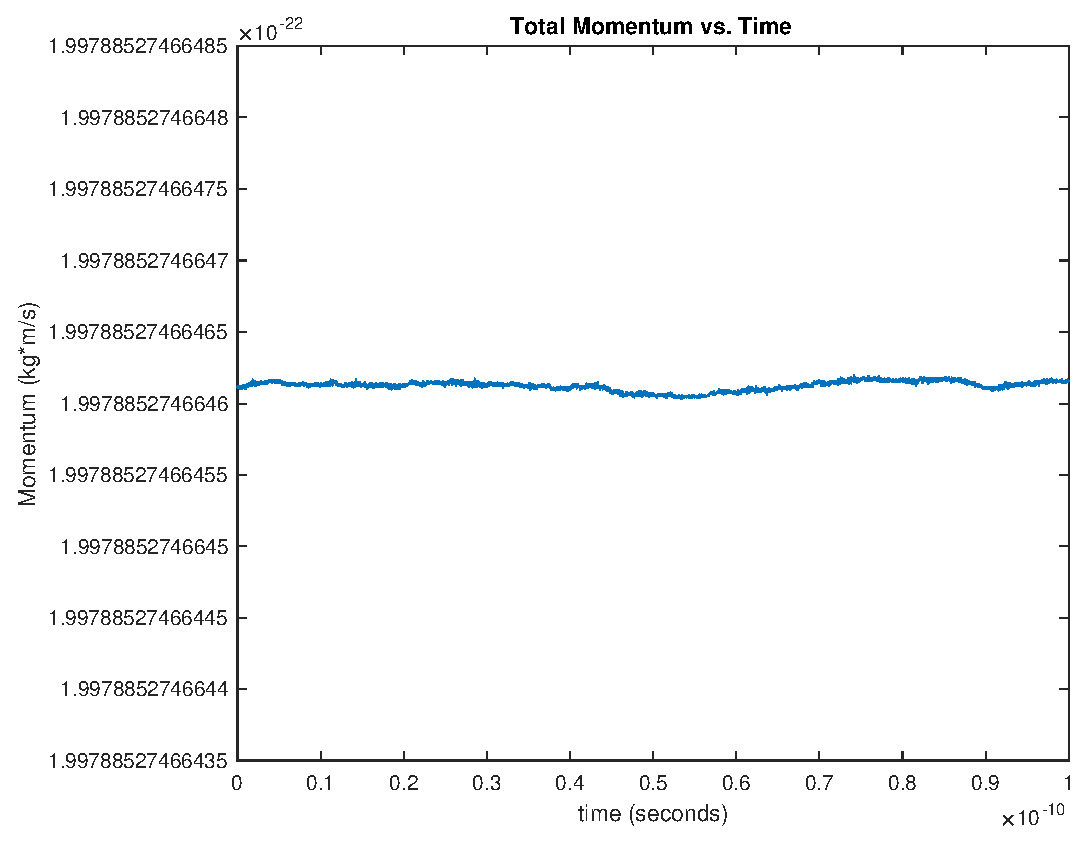
\includegraphics[width=0.9\linewidth]{./finalpics/LJPvsT.eps}
\caption{\label{LJPconservation}}
\end{subfigure}
\caption{Plots of (a) total system energy, and (b) total momentum magnitude vs. time for a lattice of Xenon atoms in the Lennard-Jones potential.  These graphs were simulated with a temperature of 100K.  The extremely stable results show that there is only a variation in energy on the order of 0.01\% and $<$ 0.01\% for momentum.} 
\end{figure} 

Shifting instead to the resulting position data, the initial and final states of the system are shown in figs. \ref{LJinitial} and \ref{LJfinal}.  In this potential, the atoms are initialized to a lower velocity due to the low temperature (100K), and thus behave similarly to if they were to begin with zero velocity.  In the initial lattice, each atom is at a minimum $r_e$ distance apart, causing the long-range attractive force to dominate.  After this attractive force acts on the particles, the atoms move closer and experience the abrupt short-range repulsive forces.  This causes a slight contraction-expansion cycle as the atoms readjust to a more energetically favorable position.  This is clear through the plot in fig. \ref{LJaverager}, where the average displacement magnitude shows slight signs of oscillation over time as it steadily moves towards the stable orientation of particles.

%L-J INITIAL AND FINAL SCATTERS
\begin{figure}[!h]
\begin{subfigure}{0.5\textwidth}
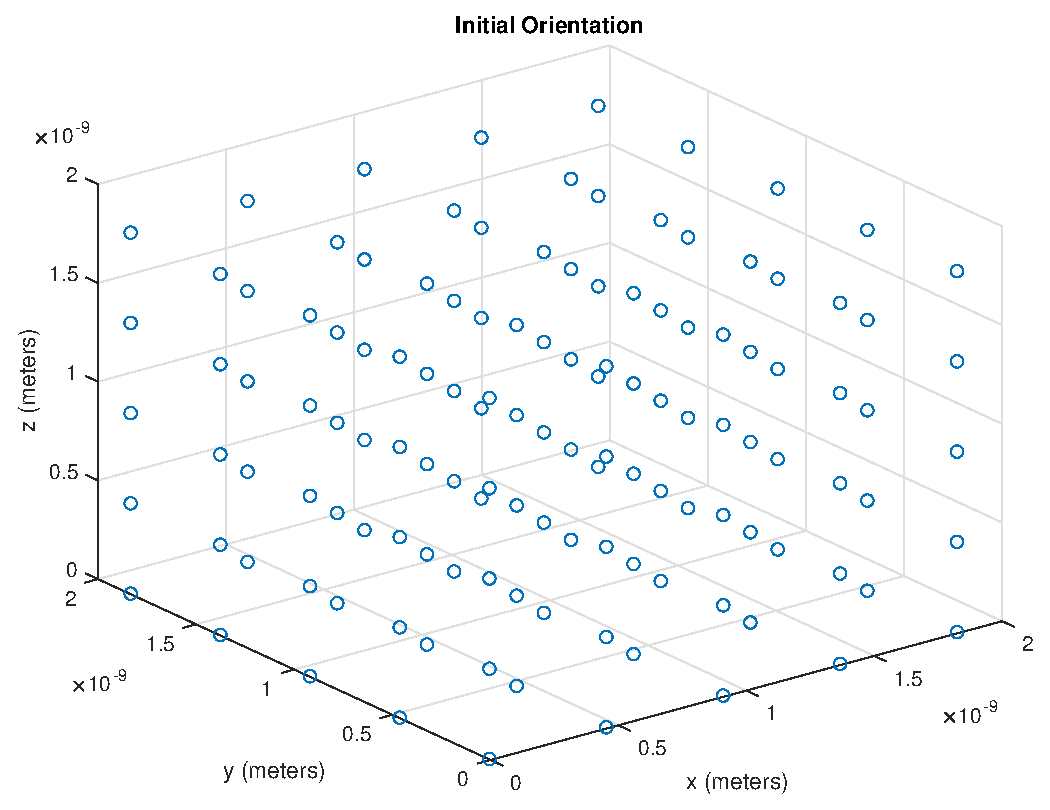
\includegraphics[width=0.9\linewidth]{./finalpics/LJinitial.eps}
\caption{\label{LJinitial}}
\end{subfigure}
\begin{subfigure}{0.5\textwidth}
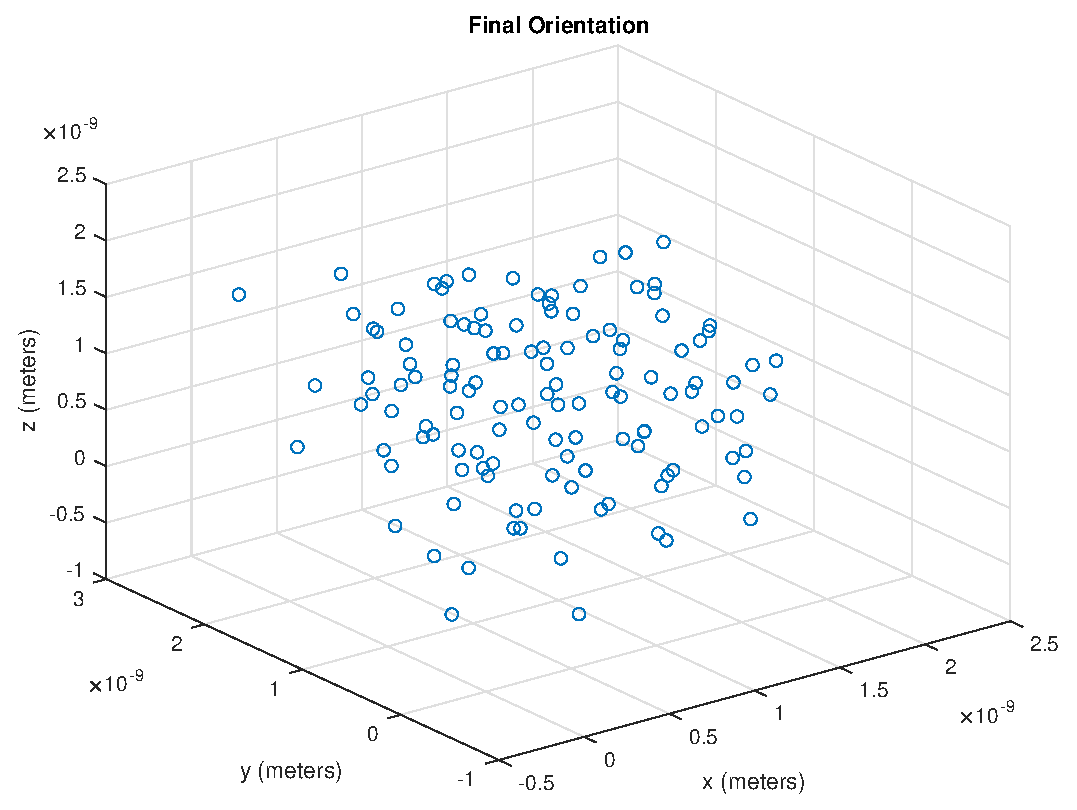
\includegraphics[width=0.9\linewidth]{./finalpics/LJfinal.eps}
\caption{\label{LJfinal}}
\end{subfigure}
\caption{3D scatter plots of (a) initial system position, and (b) final system position for Xenon atoms in the Lennard-Jones potential.  These graphs were simulated with a temperature of 100K.  The system shifts from a lattice to a more energetically favorable spherical shape, with very little evaporation.} 
\end{figure}

%L-J AVERAGE DISPLACEMENT
\begin{figure}
\begin{center}
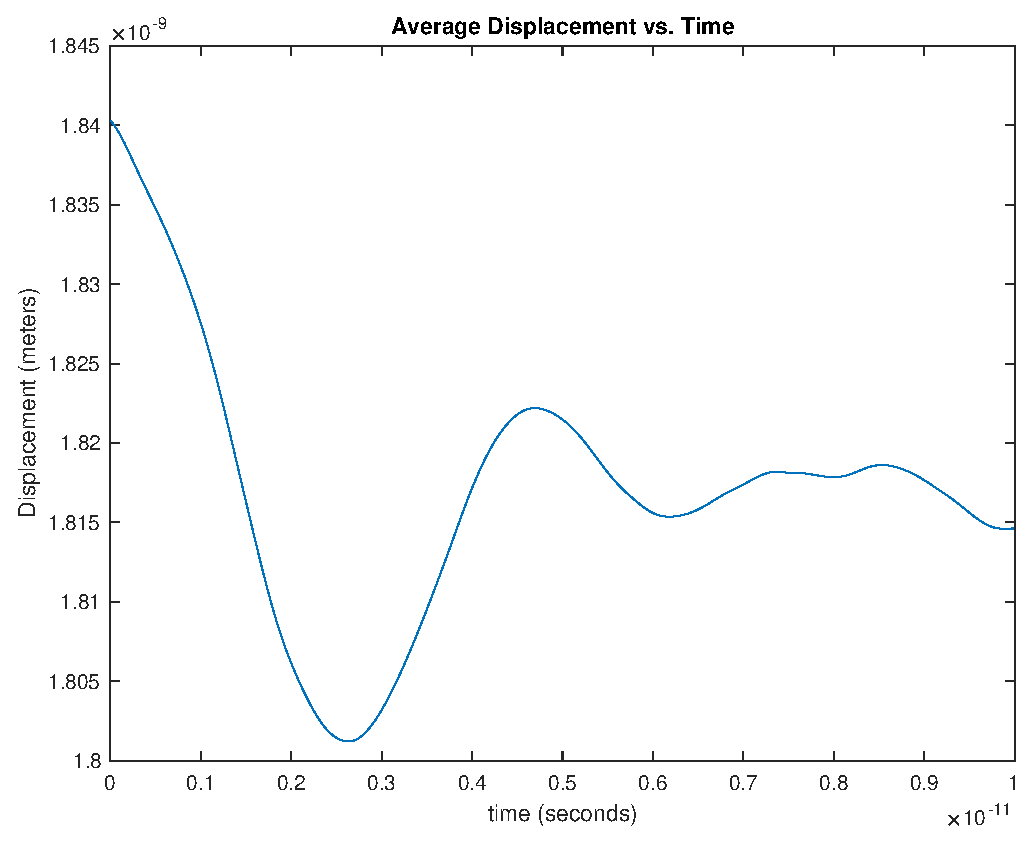
\includegraphics[width=0.5\textwidth]{./finalpics/LJaverager.eps}
\caption{\label{LJaverager} A plot of the average magnitude of the displacement from the origin over time for Xenon atoms in the Lennard-Jones potential.  As the atoms repeatedly expand and contract, there is a clear damped oscillation in the average displacement as the system settles to its final orientation.}
\end{center}
\end{figure}

\subsection*{Morse Potential}
In the Morse potential, the spring-esque behavior within the potential is again very evident.  The energy and momentum of the system are conserved with comparable accuracy on the order of $<$ 0.001\%, as seen in figs \ref{MEconservation} and \ref{MPconservation}.  This once again validates RK4, provided an acceptable timestep.

%MORSE CONSERVATIONS
\begin{figure}[!h]
\begin{subfigure}{0.5\textwidth}
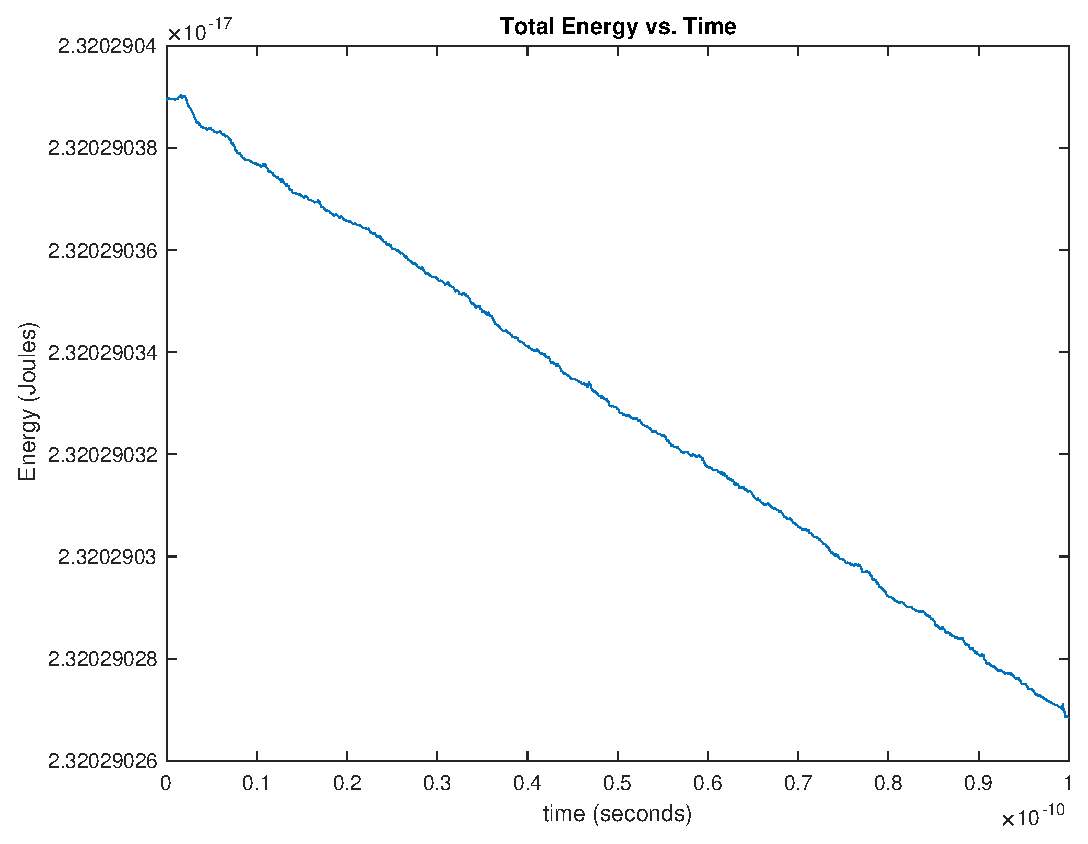
\includegraphics[width=0.9\linewidth]{./finalpics/MEvsT.eps}
\caption{\label{MEconservation}}
\end{subfigure}
\begin{subfigure}{0.5\textwidth}
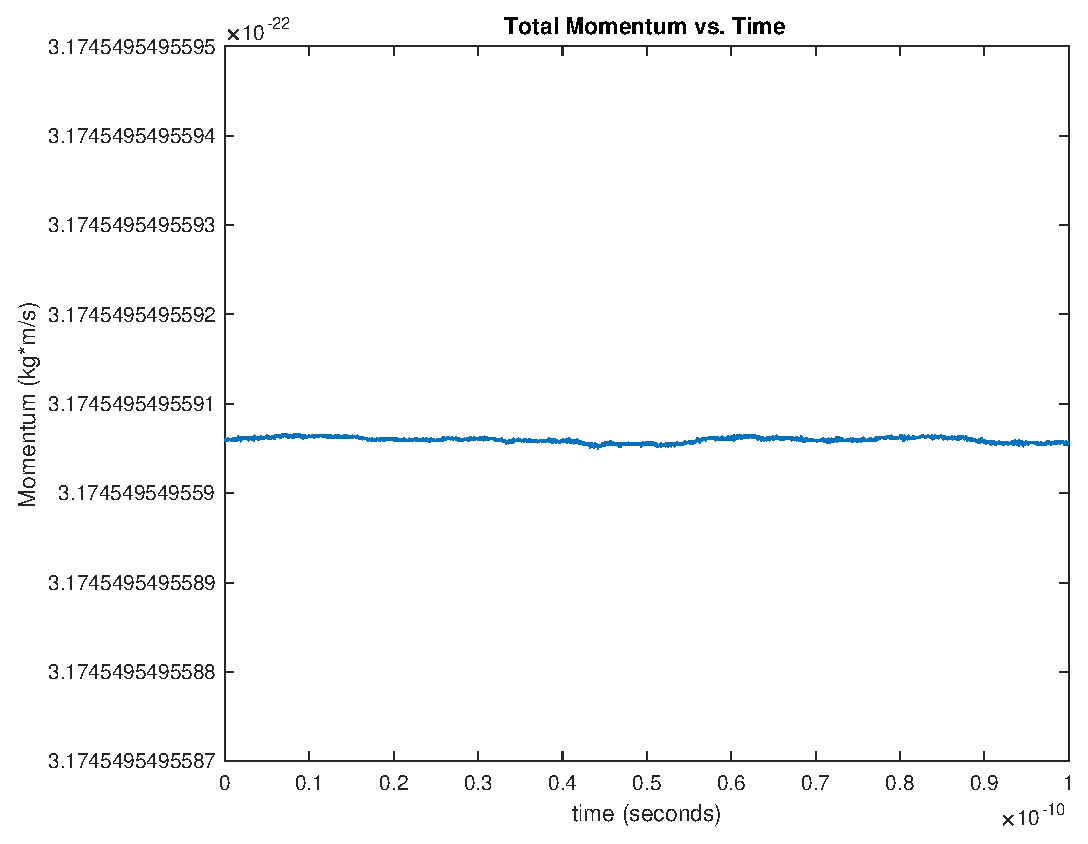
\includegraphics[width=0.9\linewidth]{./finalpics/MPvsT.eps}
\caption{\label{MPconservation}}
\end{subfigure}
\caption{Plots of (a) total system energy, and (b) total momentum magnitude vs. time for a lattice of Xenon atoms in the Morse potential.  These graphs were simulated with a temperature of 100K.  The extremely stable results show that there is a variation $<$ 0.001\% for both energy and momentum in 10000 iterative steps.} 
\end{figure}

The results of the Morse potential simulation are strikingly similar to those in the Lennard-Jones, as would be expected by the similar shapes.  Because each atom is initialized at a minimum distance $r_m$ from its neighbors, the long-range attractive force dominates.  As this force pulls the atoms inward, the short-range repulsive force acts, causing a the contraction-expansion cycle seen in the Lennard-Jones potential.  The Morse potential, however, exhibits noticeably larger oscillations, perhaps owed somewhat to the flexibility in the width parameter $a$ that does not exist in the Lennard-Jones.  This pattern is clear in fig. \ref{Maverager}, which displays the average magnitude of the displacement through the 10000 iterative steps.

%MORSE INITIAL AND FINAL SCATTERS
\begin{figure}[!h]
\begin{subfigure}{0.5\textwidth}
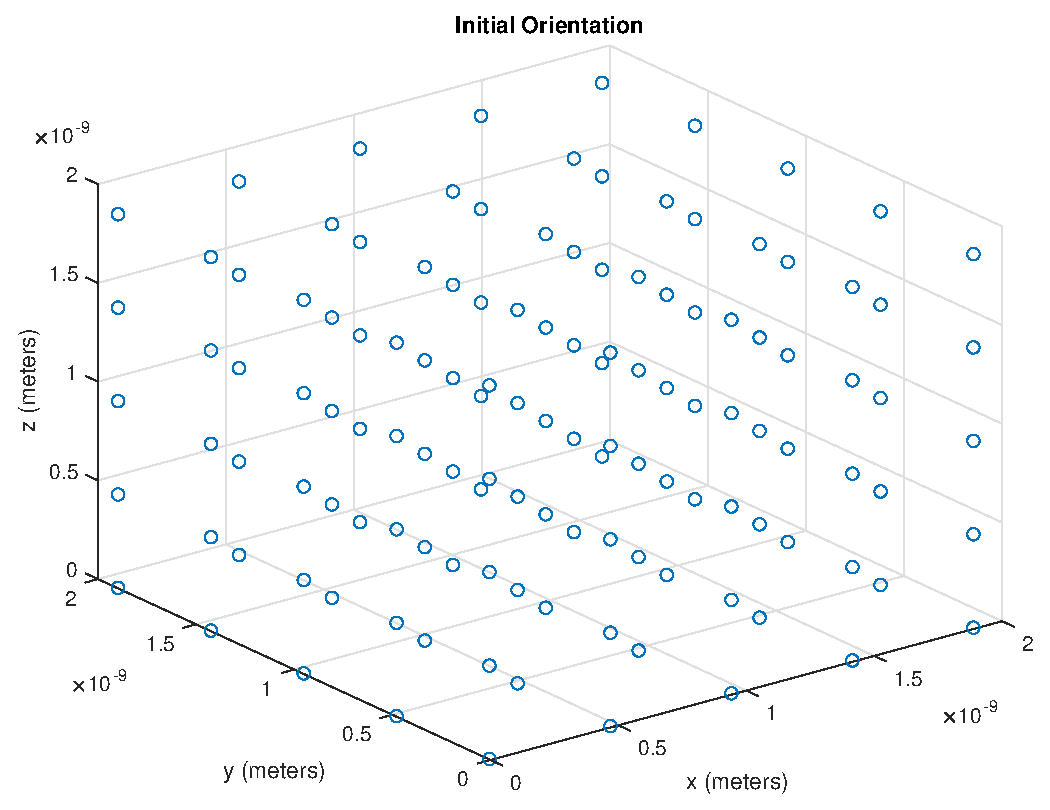
\includegraphics[width=0.9\linewidth]{./finalpics/Minitial.eps}
\caption{\label{Minitial}}
\end{subfigure}
\begin{subfigure}{0.5\textwidth}
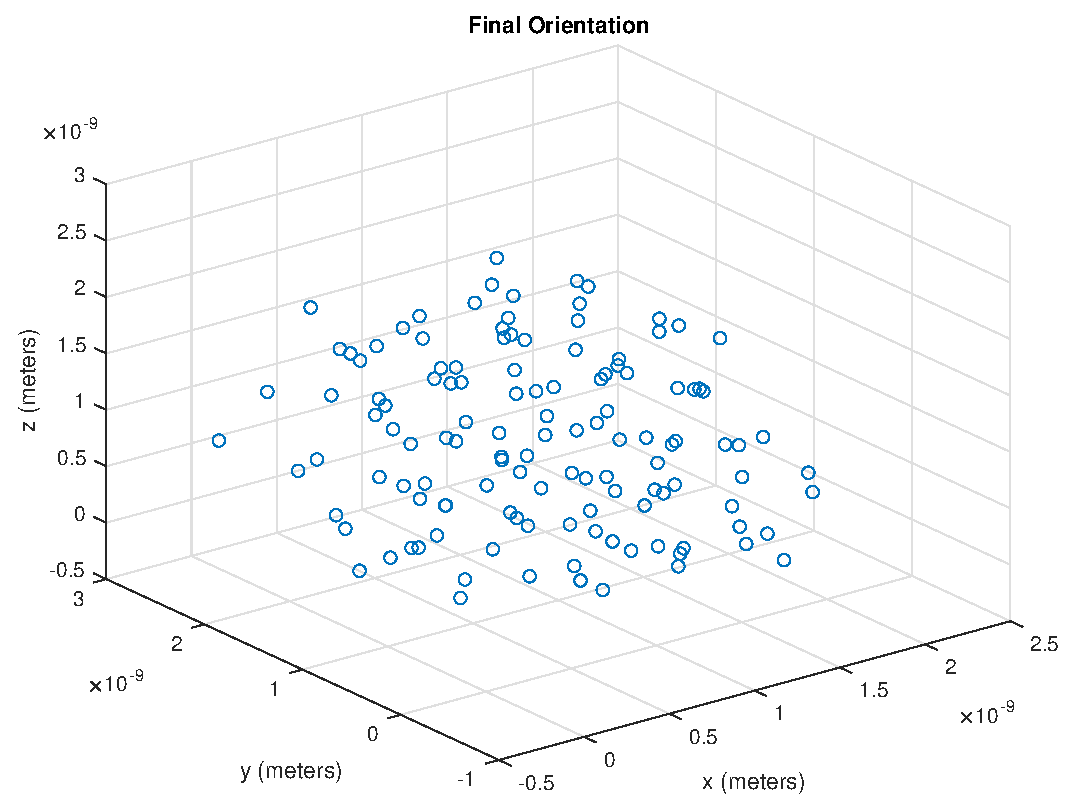
\includegraphics[width=0.9\linewidth]{./finalpics/Mfinal.eps}
\caption{\label{Mfinal}}
\end{subfigure}
\caption{3D scatter plots of (a) initial system position, and (b) final system position.  These graphs were simulated with a temperature of 100K.  The system shifts from a lattice to a more energetically favorable spherical shape with little evaporation at this temperature, as expected.} 
\end{figure}

%MORSE AVERAGE DISPLACEMENT
\begin{figure}
\begin{center}
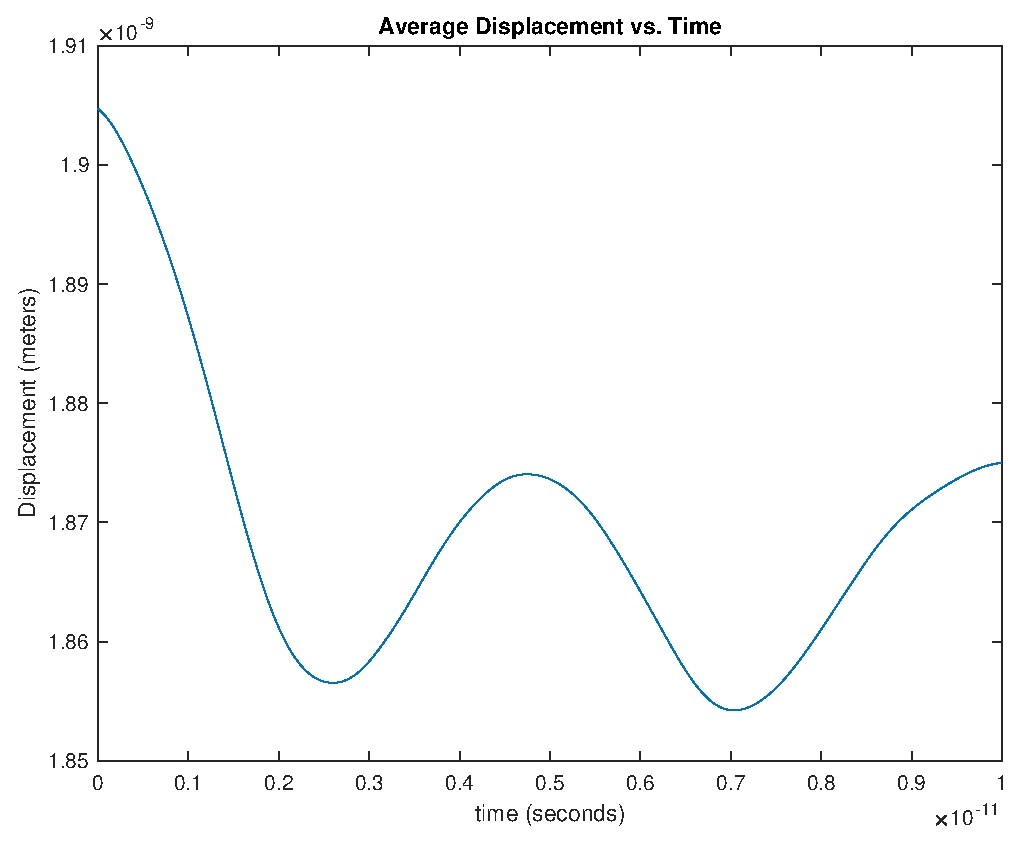
\includegraphics[width=0.5\textwidth]{./finalpics/Maverager.eps}
\caption{\label{Maverager} A plot of the average magnitude of the displacement from the origin over time for Xenon atoms in the Morse potential.  As was seen in the Lennard-Jones potential, the atoms repeatedly expand and contract, creating an oscillation in the average displacement magnitude.}
\end{center}
\end{figure}

\subsection*{Temperature Considerations}
In both potentials, the initial velocity in each direction for each atom was drawn from the Maxwell velocity distribution.  This distribution inherently depends on temperature, and therefore as we increase the temperature, the standard deviation of our initial velocity also increases.  This is to be expected, as the Maxwell velocity distribution is merely a normal distribution with $\mu = 0$ and $\sigma = \sqrt{\frac{K_bT}{m}}$.

The direct result is the evaporation of more atoms in the system as temperature increases, as shown in the figs. \ref{LJfinal1000}, \ref{LJaverage1000}, \ref{Mfinal1000}, and \ref{Maverage1000}.  The upward trend in the average displacement indicates a trend of general evaporation upon initialization, where most atoms are initialized with enough kinetic energy to effectively ``escape" the long-range attractive force of the other atoms in the system.  Both Morse and Lennard-Jones exhibit this behavior, however, the Morse potential shows faster evaporation, likely caused by the flexibility in width parameter $a$.

\begin{figure}[!h]
\begin{subfigure}{0.5\textwidth}
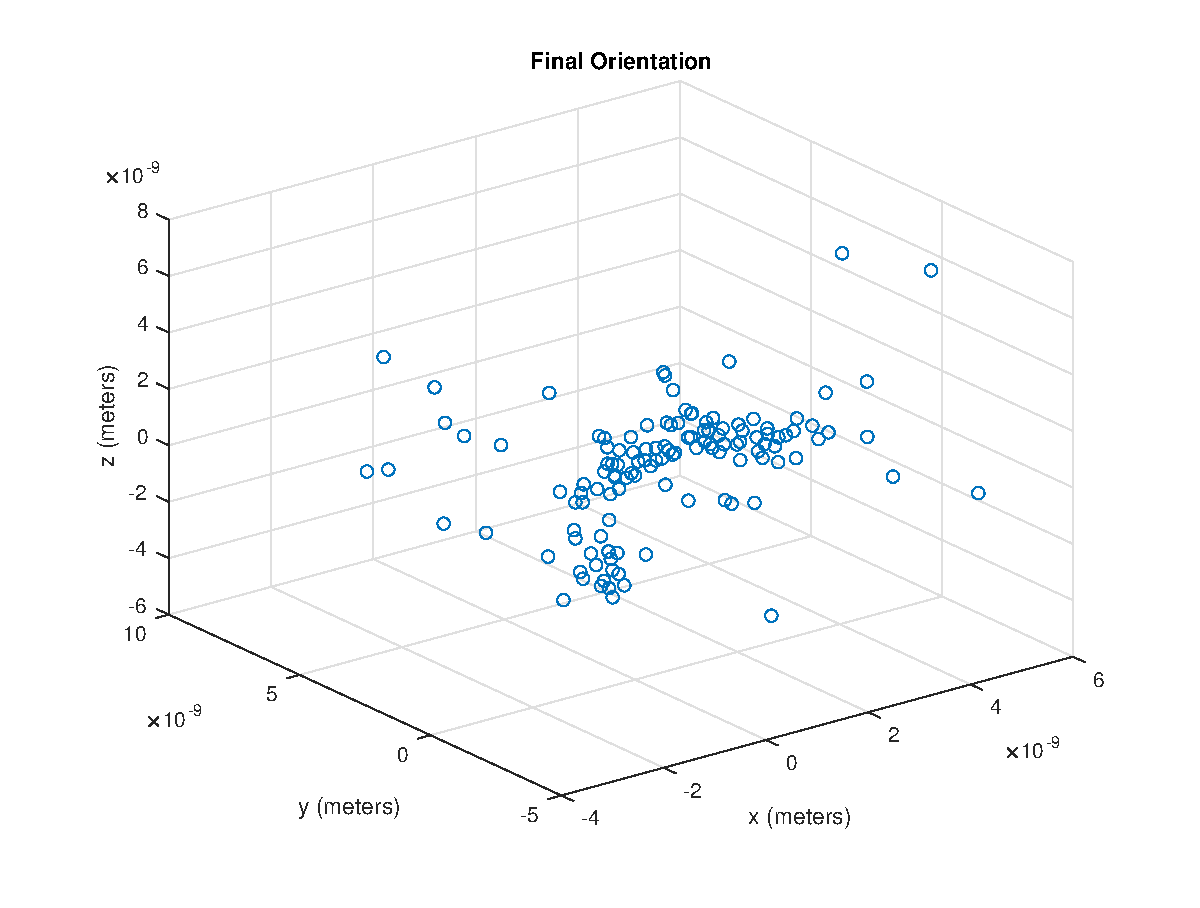
\includegraphics[width=\linewidth]{./finalpics/LJfinal1000.eps}
\caption{\label{LJfinal1000}}
\end{subfigure}
\begin{subfigure}{0.5\textwidth}
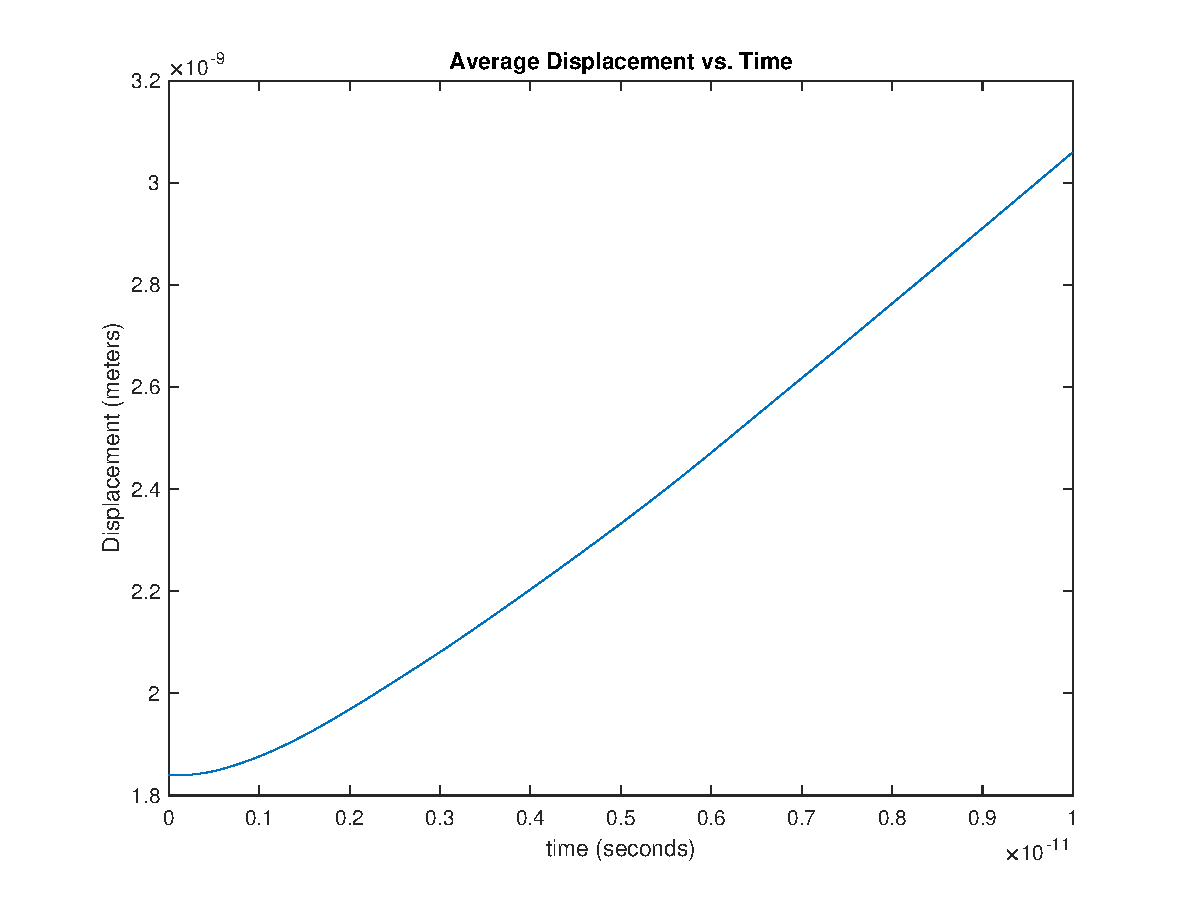
\includegraphics[width=\linewidth]{./finalpics/LJaverager1000.eps}
\caption{\label{LJaverage1000}}
\end{subfigure}
\caption{A 3D scatter plot of the final position (after $10^{-11}$ seconds) of a Xenon lattice in the Lennard-Jones potential (a) and the average magnitude of the displacement over time (b)  when initialized to 1000K.  It is clear from both plots the increased temperature causes more atoms to have enough energy to leave the initial lattice and evaporate.} 
\end{figure}

\begin{figure}[!h]
\begin{subfigure}{0.5\textwidth}
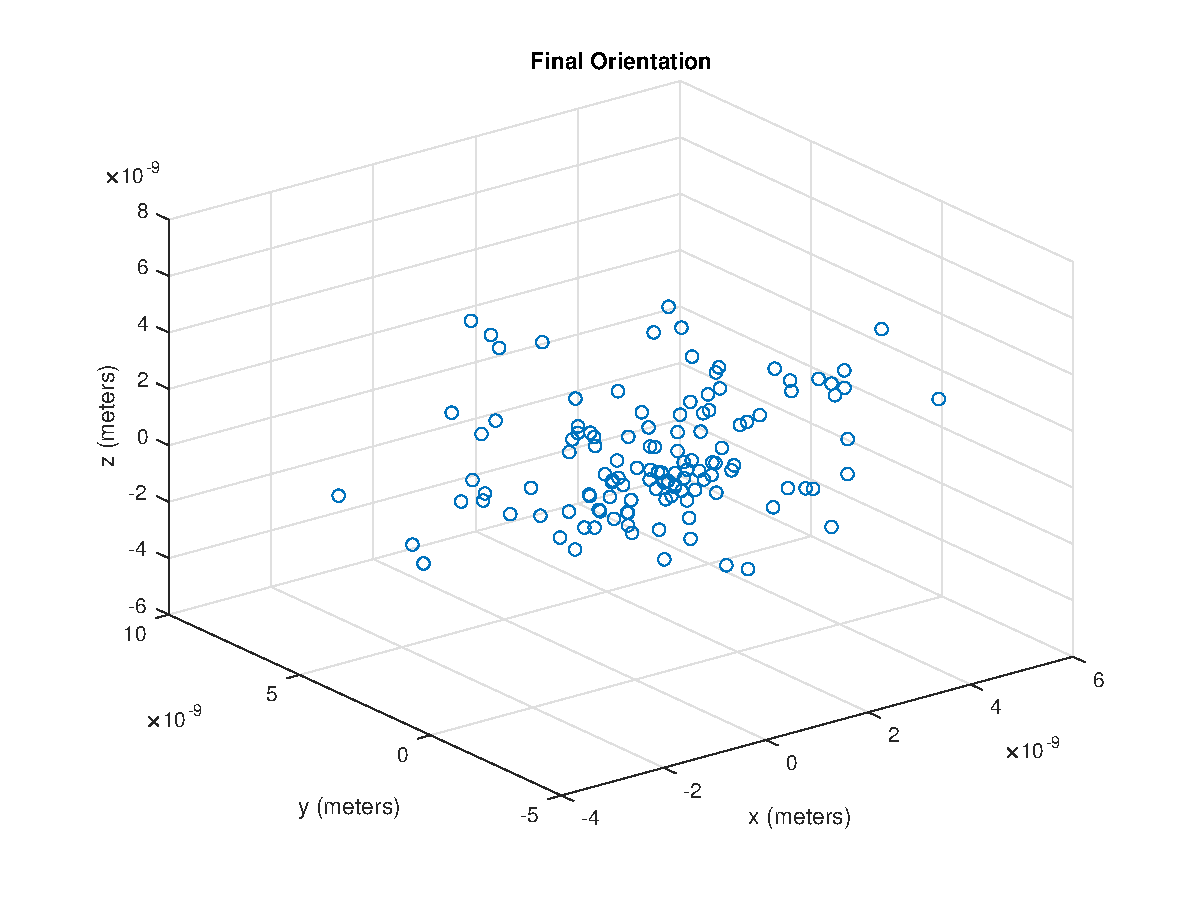
\includegraphics[width=\linewidth]{./finalpics/Mfinal1000.eps}
\caption{\label{mfinal1000}}
\end{subfigure}
\begin{subfigure}{0.5\textwidth}
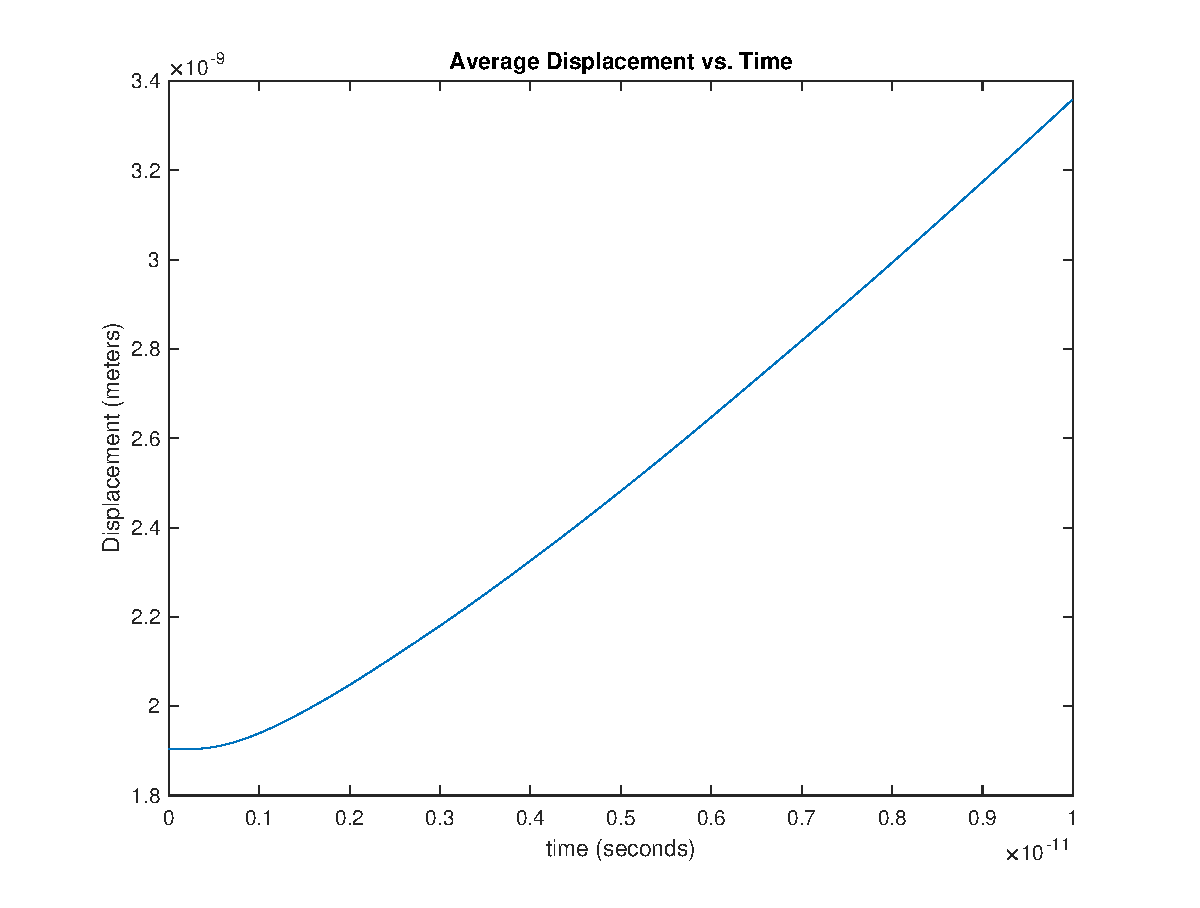
\includegraphics[width=\linewidth]{./finalpics/Maverager1000.eps}
\caption{\label{maverage1000}}
\end{subfigure}
\caption{A 3D scatter plot of the final position (after $10^{-11}$ seconds) of a Xenon lattice in the Morse potential (a) and the average magnitude of the displacement over time (b)  when initialized to 1000K.  It is clear from both plots the increased temperature causes more atoms to have enough energy to leave the system entirely and evaporate.} 
\end{figure}

Another noteworthy effect of temperature is the structural order that appears at lower temperature.  As Xenon shifts from gas, to liquid, to solid, it gains more structural order, and therefore has an inverse relationship with temperature.  To analyze this order, histograms of the final distance to neighbors in multiple simulations have been plotted in figs. \ref{LJrel}, \ref{LJrelhigh}, \ref{Mrel}, and \ref{Mrelhigh}.  These histograms effectively plot the distribution of distances between each atom and its neighbors. The sharp peaks throughout at low temperatures are caused by lower temperatures creating lower kinetic energies and therefore a lower probability of escaping the potential wells.  As the system is heated, some atoms have a higher probability of enough kinetic energy (velocity) to overcome the potential well and evaporate, eliminating the short range order at higher temperatures..

\begin{figure}[!h]
\begin{subfigure}{0.5\textwidth}
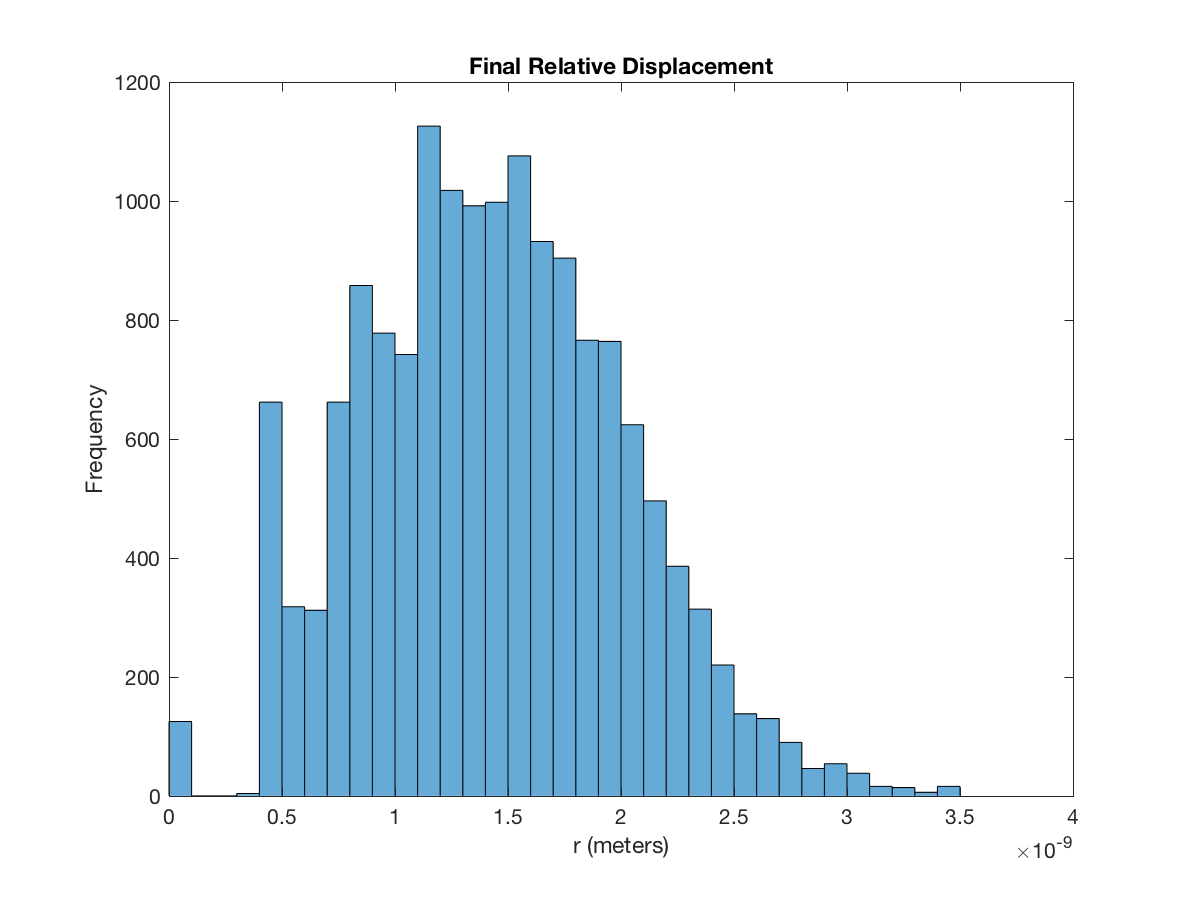
\includegraphics[width=0.9\linewidth]{./finalpics/LJfinalrelativer.eps}
\caption{\label{LJrel}}
\end{subfigure}
\begin{subfigure}{0.5\textwidth}
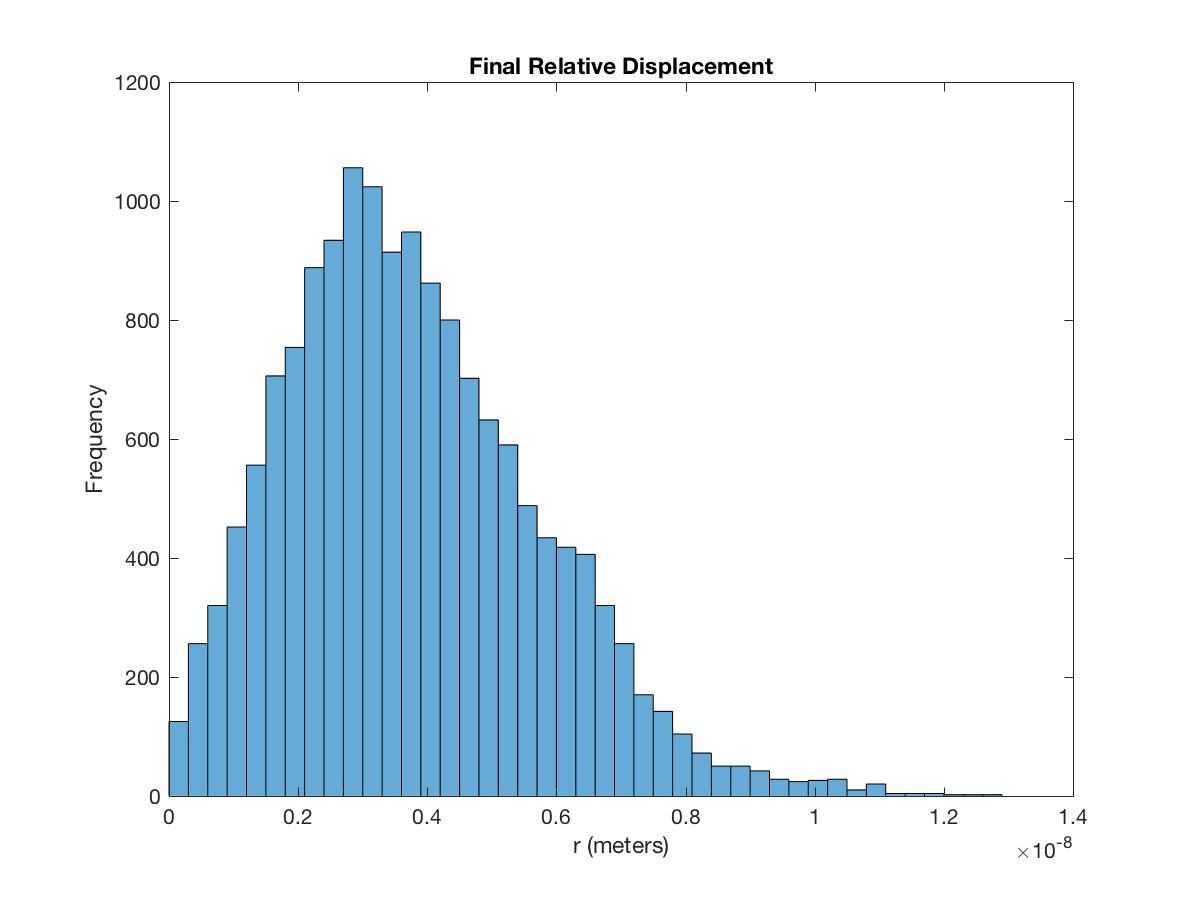
\includegraphics[width=0.9\linewidth]{./finalpics/LJrel1000.eps}
\caption{\label{LJrelhigh}}
\end{subfigure}
\caption{Histograms of the relative distance to all other particles in the system at (a) 100K, and (b) 1000K in the Lennard-Jones potential.  Definite peaks occur at low temperatures across short and long range, and as the element transitions to liquid and gaseous phases, the long range order dissipates.} 
\end{figure}

\begin{figure}[!h]
\begin{subfigure}{0.5\textwidth}
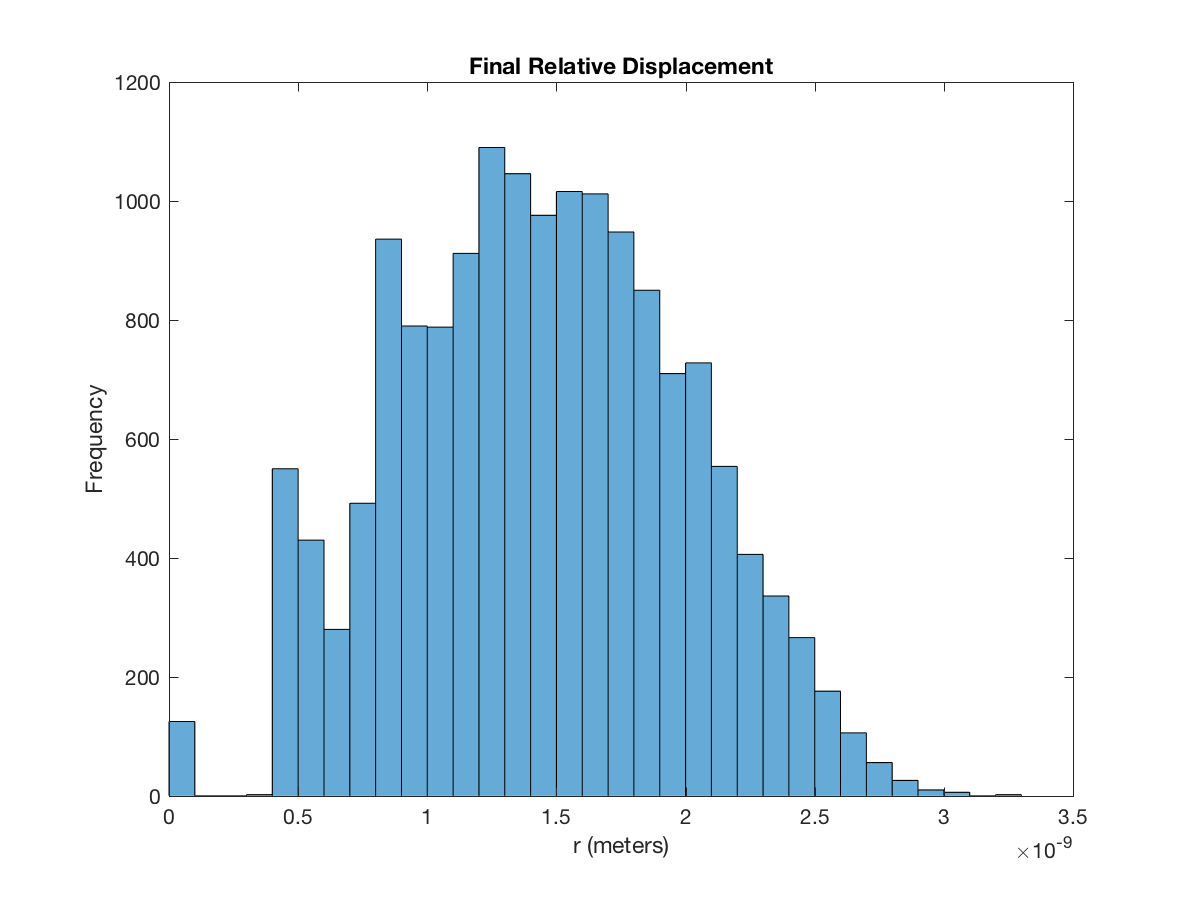
\includegraphics[width=0.9\linewidth]{./finalpics/Mfinalrelativer.eps}
\caption{\label{Mrel}}
\end{subfigure}
\begin{subfigure}{0.5\textwidth}
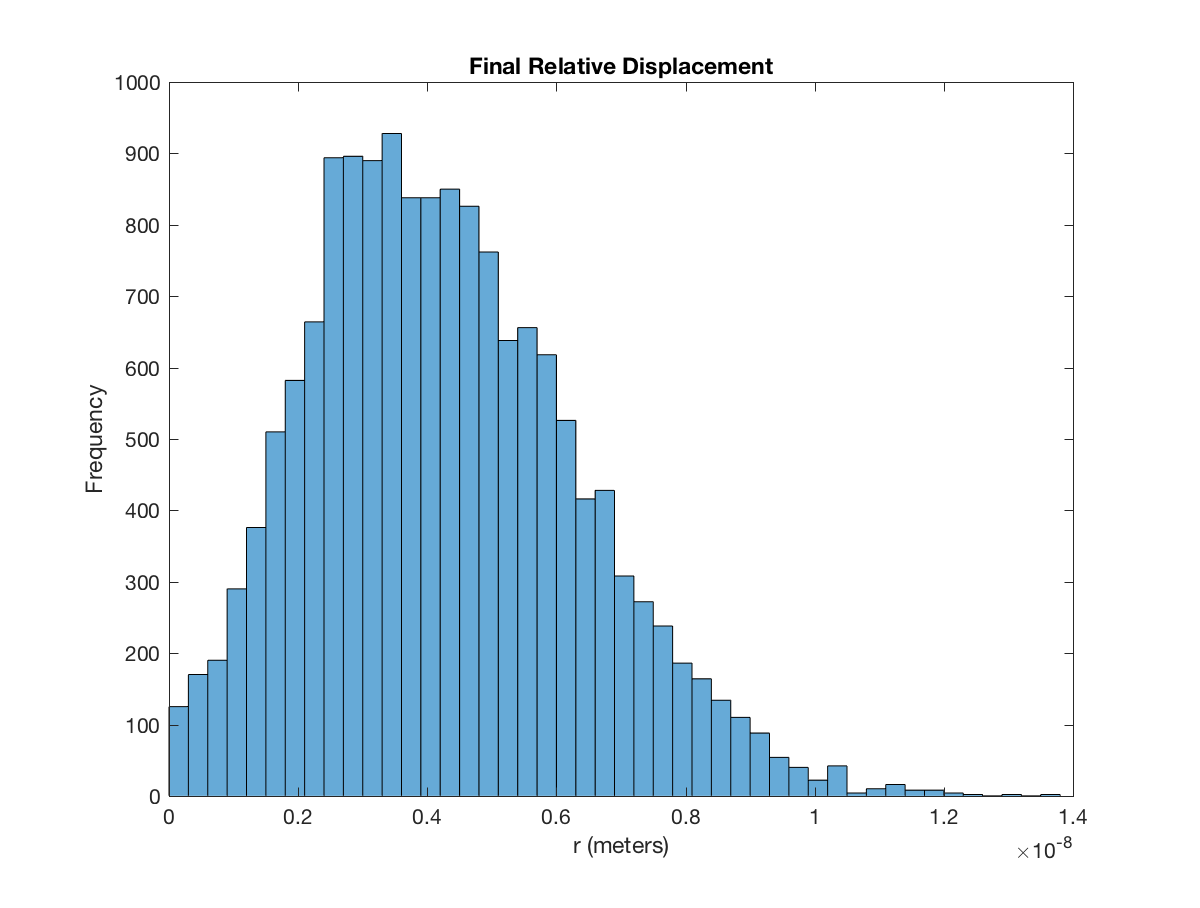
\includegraphics[width=0.9\linewidth]{./finalpics/Mrel1000.eps}
\caption{\label{Mrelhigh}}
\end{subfigure}
\caption{Histograms of the relative distance to all other particles in the system at (a) 100K, and (b) 1000K in the Morse potential.  Definite peaks occur at low temperatures across short and long range, and as the element transitions to liquid and gaseous phases, the long range order dissipates.}
\end{figure}

\subsection*{Comparison to Verlet Integration}
Fourth-order Runge-Kutta, while highly precise, is incredibly computationally exhaustive.  Where simpler methods such as Verlet integration only involve performing full iterative calculations of the force and positions twice per timestep, each run through the RK4 algorithm involves averaging three additional values each with new force and position calculations.

This repetition in mind, the average runtime of the RK4 algorithm is approximately three times longer than the runtime of the previously written Verlet integration method for solving the same system's equations of motion. \autocite{me}  Both codes have been modified to output the total time used in calculation before and after the algorithms begin by calling the 'system\_clock' subroutine before and after calculation.  The subroutine also provides the number of 'ticks' per second, and this value is used to find the total runtime of each program in seconds.

\begin{table}[h!]
\begin{center}
\begin{tabular}{|c|cc|}
\hline
\quad & Lennard-Jones Runtime (s) & Morse Runtime (s) \\
\hline
RK4 & 23.334 & 25.926 \\
Verlet & 8.422 & 7.322\\
\hline
\end{tabular}
\end{center}
\label{runtimes}
\caption{A table detailing the average runtime of n-body simulations using both RK4 and Verlet integration methods.  The averages were collected over 10 runs each using 10000 timesteps of $10^{-14}$.  Simulation runs were performed back to back, with no change in background programs running on system between simulations.}
\end{table}

The average runtimes are compared in \ref{runtimes}.  The Morse potential generally takes longer to compute, likely because of the double-precision exponential functions that are required in the calculation.  As expected, the RK4 algorithm takes on the order of 300\% the amount of time as the Verlet integration algorithm.  Arguably the improvement in precision does not merit the time in this scenario, however, in cases where small error can quickly propogate over longer iteration times, RK4 may be necessary.
\subsection*{Discussion}
The results of these simulations justify the use of RK4 as an integration method, provided an adequate time step.  There is of course numerical error associated with the calculations, however the variance in energy below 0.01\% gives evidence to the method's overall accuracy.  RK4 also provides more precise results than Verlet integration, at the cost of high computation times. \autocite{me}  Both the Lennard-Jones and Morse potentials induce the expansion-contraction cycles in the simulation results, causing a similar system to bodies connected by springs. \autocite{mpotential,ljpotential} The introduction of temperature dependence of the initial velocities for the lattice of Xenon atoms shows the transition between ordered (solid) and unordered (liquid, gaseous) phases of the material.
\newpage
\section*{Acknowledgements}
I would like to thank Dr. Justin Oelgoetz for assistance formulating the simulation code, and for providing insightful explanations and troubleshooting along the way.

The ``random\_number" subroutine within the code was seeded using an algorithm provided by Justin Oelgoetz, as sourced from open source code online.  This code seeds Fortran's random number generator to create pseudo-random numbers that are unique to each run.

All graphs and plots made in this paper were produced using MATLAB computational software.
\newpage

\printbibliography
\newpage
\section*{Appendix}
Attached is the source code for this project, written in Fortran.
\subsection*{Main}
\lstinputlisting[language=Fortran]{../nbodyrk4.f90}
\subsection*{Morse Potential Module}
\lstinputlisting[language=Fortran]{../morse.f90}
\subsection*{Lennard-Jones Potential Module}
\lstinputlisting[language=Fortran]{../lennardjones.f90}
\subsection*{Constants Module}
\lstinputlisting[language=Fortran]{../constants.f90}
\subsection*{MATLAB Plotting Script}
Code can be run while MATLAB is in the directory containing result files and will create a .gif file of positions, total energy and momentum plots, an initial velocity sampling histogram, average displacement magnitude vs. time, and initial and final scatter plots of position and save them to the directory.
\lstinputlisting[language=Octave]{../plots.m}
\end{document}